\chapter{Choice of model parameters}

\section{Selection of dynamical reputation model parameters}

One of the largest drawbacks of DIBRM is the parameter tuning problem. In previous applications of the model \cite{melnikovDynamicInteractionBasedReputation2018,yashkina2020} there was no single best set of parameter values for modeling dynamic reputation in Stack Exchange communities. For example, in \cite{yashkina2020} the best approximation of the official Stack Exchange reputation is obtained with $t_a =2, \beta = 1, \alpha = 1.4$ which means there is no active forgetting factor. In our application of DIBRM to SE communities we opted for a different set of parameter values. Details of parameter search and tuning are presented in SI.

For basic reputation contribution of a single interaction we selected $I_{bn} = 1$ and at the same time this is the threshold value of an active user. This value is intuitive as every interaction has initial contribution of +1 to user's reputation, although the previous works have used values of +2 and +4. Following the previous work and after examining the median/average time between subsequent interactions of the same user, we selected $t_a = 1$, which also means that reputation in our model will be updated every day during the time-window of the analysis, regardless of whether the user is active or not. To emphasize the bursts of activity and frequent recent interactions, cumulative factor has a larger value $\alpha = 2$. Finally, the most delicate parameter is the forgetting factor, which at the same time determines the weight of past interactions and the reputational punishment due to user inactivity. Here we need to select the value of parameter $\beta$ so we include the forgetting due to inactivity but not to penalize is too much. In Fig. A1 we show how different values of parameter $\beta$ influence the time needed for user's reputation to fall on value $I_{n}=1$ due to user's inactivity and value of dynamical reputation in the moment of the last activity. The higher the value of parameter $\beta$ and initial dynamical reputation of users, the longer time it takes for user's reputation to fall on baseline value. For parameter $\beta=0.9$ and $I_{n}=5$, user's reputation falls on value $I_{n}=1$ after less than 20 days, while this time is doubled for $\beta=0.96$. We see, that for higher values of parameter $\beta$ the time needed for $I_{n}$ to fall on value $1$ becomes longer, and that the the initial value of reputation becomes less important. 

Figure A2 in SI shows the difference between the number of users that had at least one activity in the window of 30 days and number of users with reputation higher than $1$ during the same period for different values of parameter $\beta$. The minimal difference between these two variables is observed for the values of $\beta$ between $0.94$ and $0.96$ for both live and closed communities. Since we want to compare communities, we select $\beta = 0.96$ after verifying that this level of reputational decay does not reduce the number of active users (based on their dynamic reputation) below the actual number of users who have been active (interacted with the community) in the time window of 30 days. 

%To summarize, our model of dynamical reputation has three parameters: 1) basic reputation contribution $I_{bn}=1$; 2) cumulative factor $\alpha=2$; 3) forgetting factor $\beta=0.96$. The selected values of parameters are used for measuring dynamical reputation of user in all four pair SE communities. Given these values of parameters, the minimal reputation achieved by the user immediately after they have made an interaction in the SE community is $1$. This reputation will decay below $1$ if the user does not perform another interaction within the one-day time window. For any user in a community, when their reputation drops below $1$, we consider this user inactive which means that the user at that time is not "visible" in the community and their past contributions at that time are unlikely to impact other users. The number of active users and mean user reputation for different Stack Exchange communities are shown in Fig. \ref{fig:dr6panel}.


\section{Dynamic reputation - $\beta$ parameter}

Our implementation of dynamic reputation model was based on $\beta = 0.96$. There are several reasons for selecting this value.

In Dynamic reputation model, the $\beta$ parameter controls the strength of the forgetting fator of the model.  The value of this parameter should reflect the core feature of the reputational systems and make reputation easier to loose. Due to user's inactivity, any level of reputation will eventually decay to below 1. Dependence of time needed for reputation to drop below this level and the $\beta$ parameter, as well as reputation before inactivity is shown on Figure~\ref{fig:betadelta}. Here $I_n$ is equal to the raw number of interactions in the community without forgetting or cumulative factor at work.

%\begin{figure}[h!]
%	\centering
%	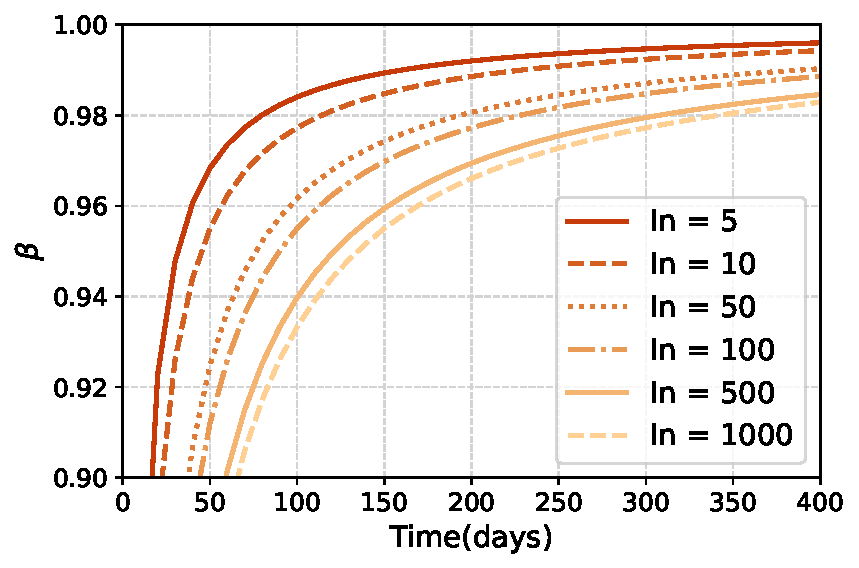
\includegraphics[width=0.5\linewidth]{figures/stackexchange/reputation_decay.pdf}
%	% REMOVE 'SLOWER' FROM THE PLOT TITLE > zamenjeno i formulu sam prebacila u caption
%	\caption{Dependence of parameter $\beta$ and number of days $\Delta$ needed for reputation $I_n$ to drop to $I_{n_0} = 1$. Dependence of parameter $\beta$ and number of days when reputation due inactivity decreases from $I_n$ to $I_0$ is given as  $\beta = (\frac{I_{n0}}{I_{n}})^{(1/\Delta)}$ }
%	\label{fig:betadelta}
%\end{figure}

\begin{figure}[h!]
	\centering
	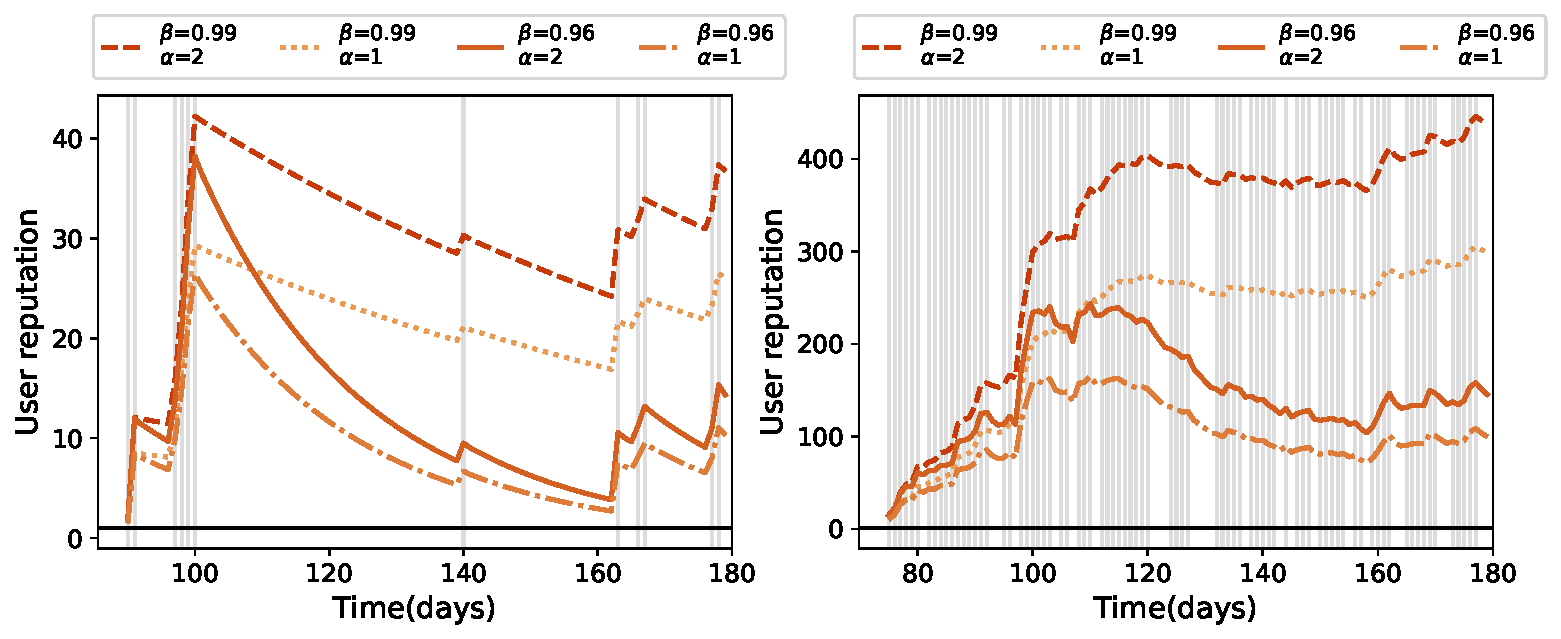
\includegraphics[width=0.8\linewidth]{figures/stackexchange/single_user_reputation.pdf}
	% REMOVE 'SLOWER' FROM THE PLOT TITLE > zamenjeno i formulu sam prebacila u caption
	\caption{Single users reputations }
	\label{fig:singleuser}
\end{figure}

For $\beta$ values below 0.96, the decay is fast and within two to four months of inactivity even high values of reputation are reduced below the threshold. On the other hand, with $\beta$ values the decay proces is more differentiated and high reputation becomes harder to loose, surviving up to a year of inactivity. For $\beta$ equal to 0.96, it takes a month for reputation based on 5 interactions to decay and around five months for high reputation based on 500 or 1000 interactions to decay below the threshold.

\textbf{30 days sliding window} We compared the number of users with estimated reputation higher than 1 for different parameters $\beta$ and concluded that $\beta$ close to $0.96$ approximates the number of users with recorded interactions in a given 30 days sliding window. For each pair of communities we calculated number of users with at least one interactions in every 30 days sliding window and then we estimated several times series expressing the number of users with reputation higher than 1 for fixed $\beta$. Then we calculated the root mean square error (RMSE) between those time series for the first 200 days. Values of RMSE are shown on Figure~\ref{fig:rmse}. For each community, we can find parameter $\beta$ that minimizes RMSE. Although $\beta$ does not have a unique value across communities, it varies between 0.95 and 0.96. 
%We should notice that taking different time period, for example, the first 90 days, we can get different optimal values of betta, but they'll probably take values between 0.95 and 0.96 (I can test it). 


\begin{figure}[h!]
	\centering
	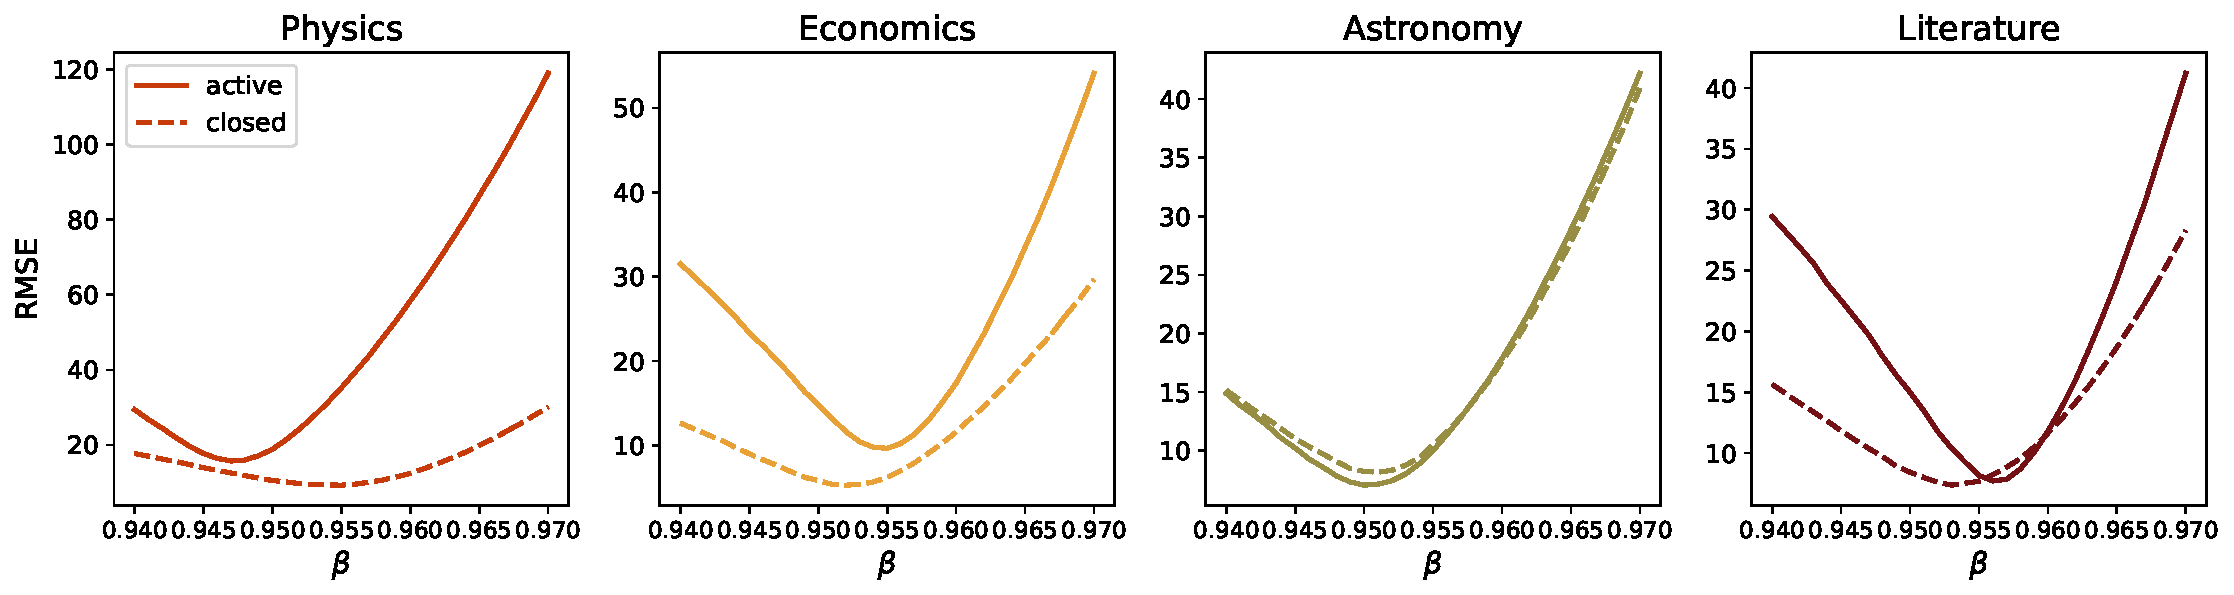
\includegraphics[width=\linewidth]{figures/stackexchange/rmse.pdf}
	\caption{RMSE between number of active users in sliding window of 30 days and number of users with reputation $>1$ for  $0.94< \beta <0.97$ with step $0.001$. }
	\label{fig:rmse}
\end{figure}

Figure \ref{fig:nusers} shows comparison between number of users in 30 days sliding window, number of users for these optimal values $\beta = 0.954$ and $\beta =0.96$. For $\beta = 0.96$ we observe that in most communities estimated number of active users consistently slightly higher than the actual number of users which have made at least one interaction in that sliding window. This means that dynamic reputation model in some cases overestimates the reputation of the user, but far more important is that it never understimates the real number of active users. Since we base our calculations of total and average reputation within the community only on users whose reputation is higher than the threshold this is important as no active users are disregarded by the model due to the value of the decay parameter.

\begin{figure}[h!]
	\centering
	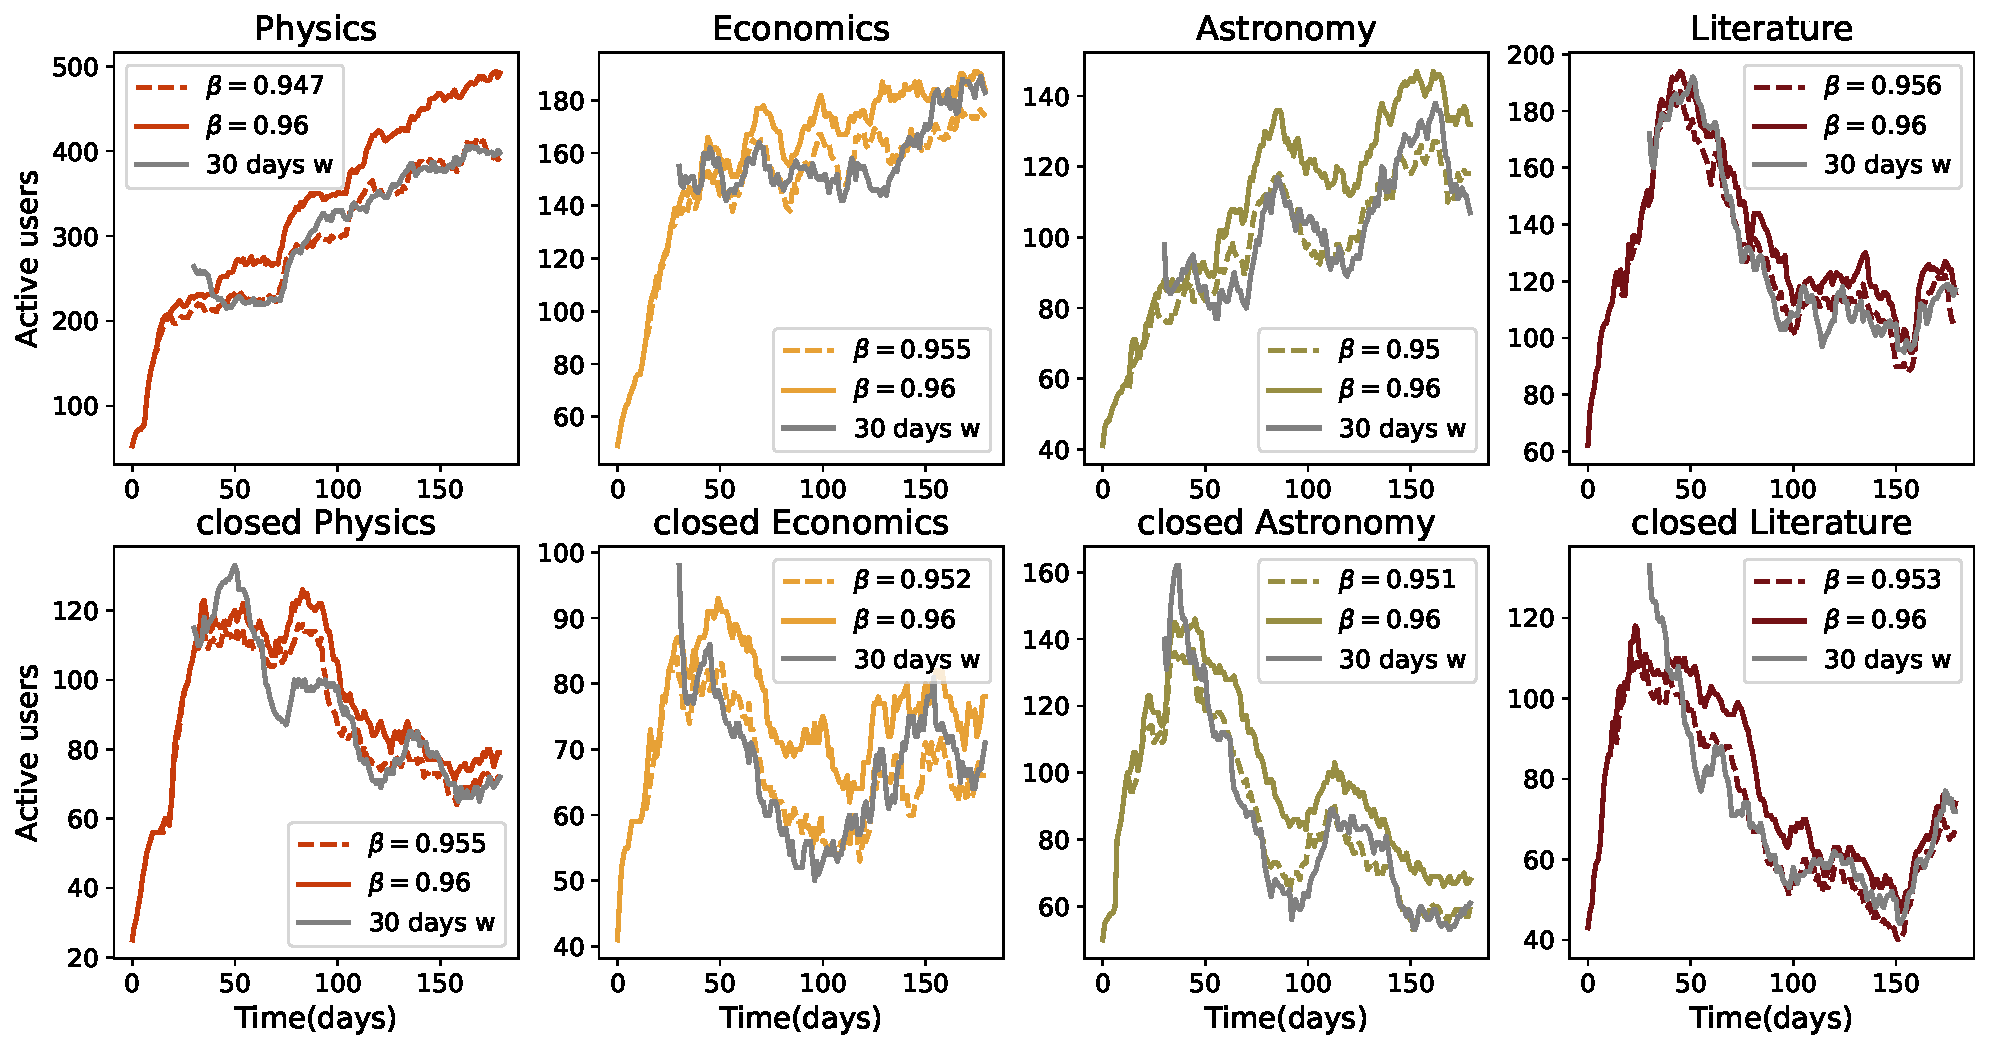
\includegraphics[width=\linewidth]{figures/stackexchange/active_users.pdf}
	\caption{Number of active users in a sliding window of 30 days and number of users with dynamic reputation higher than 1 for $\beta=0.954$ and $\beta=0.96 $ which provide the best fit to the number of users in 30 days sub-networks for each community}
	\label{fig:nusers}
\end{figure}

Finally, it's imporant that our dynamic reptuation captures the trend of long-term user activity. In Figure~\ref{fig:active-users} solid lines show the time series of estimated dynamic reputation for $\beta = 0.96$ while dashed lines show the number of users who were active in a given sliding window and continued to be active in the next one. Although the total estimated number of active users is expectedly higher, two time series follow similar trends in different communities.

\begin{figure}[h!]
	\centering
	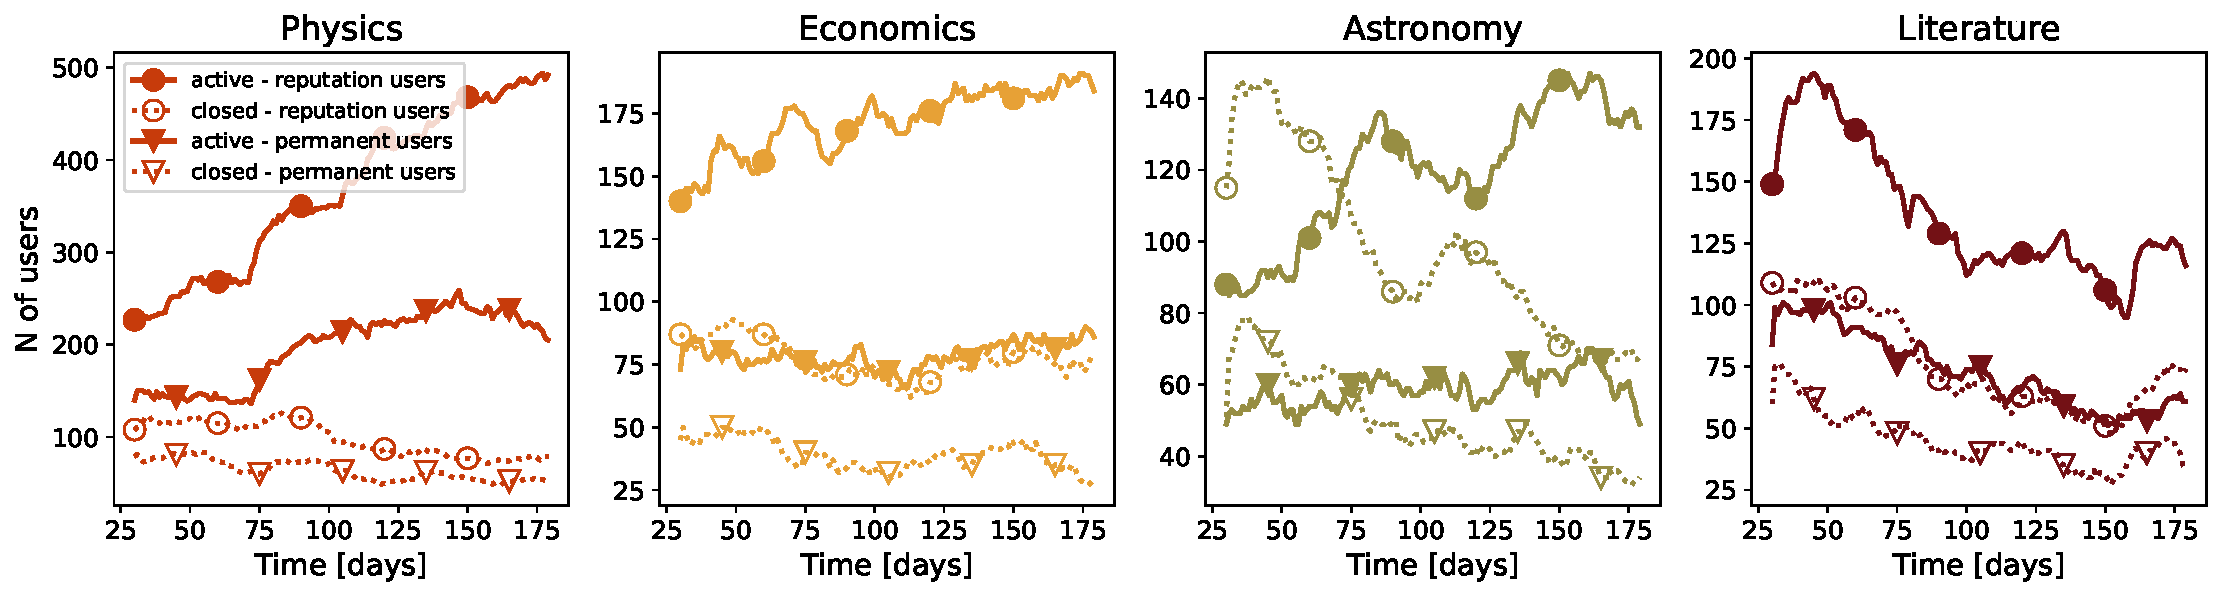
\includegraphics[width=1\linewidth]{figures/stackexchange/permanent_users.pdf}
	\caption{Solid lines represent number of users with dynamic reputation higher than 1 for $\beta=0.96$ while dashed lines are number of users within 30 days sliding window who were active and remained to be active. Blue lines are beta, while red lines are area51 communities.}
	\label{fig:active-users}
\end{figure}
\clearpage
